\documentclass[a4paper, spanish, 11pt]{article}

\usepackage[utf8]{inputenc}
\usepackage[spanish, es-tabla]{babel}
\usepackage[margin={24mm, 24mm}]{geometry}
\usepackage{amsmath}
\usepackage{amssymb}
\usepackage{float}
\usepackage{graphicx}
\graphicspath{ {res/img/} }

\begin{document}
  \thispagestyle{empty}
  \begin{itemize}

    \item \textbf{Nombre y Apellidos}: Sergio García Prado

    \item \textbf{Serie}: \texttt{weightloss} (propuesta propia extraida de internet)

    \item \textbf{Modelo Final}:

    \begin{equation*}
       \text{SARIMA}(0, 1, 1)(0, 1, 1)_{12}(0, 0, 1)_{17}
    \end{equation*}

    \begin{align*}
      \widehat{\theta}_{1} = 0.33629 &&  \widehat{\theta}_{12} = 0.62106 && \widehat{\theta}_{17} =-0.15874
    \end{align*}

    \begin{equation*}
      \begin{split}
        X_t = X_{t - 1} + &X_{t - 12} - X_{t - 13} + a_t - \theta_{1}a_{t - 1} - \theta_{12}a_{t - 12} + \theta_{1}\theta_{12}a_{t - 13} \\
        &- \theta_{17}a_{t - 17} + \theta_{1}\theta_{17}a_{t - 18} + \theta_{12}\theta_{17}a_{t - 29} - \theta_{1}\theta_{12}\theta_{17}a_{t - 30}
      \end{split}
    \end{equation*}

    \item \textbf{Residuales}:

    \begin{figure}[H]
      \centering
      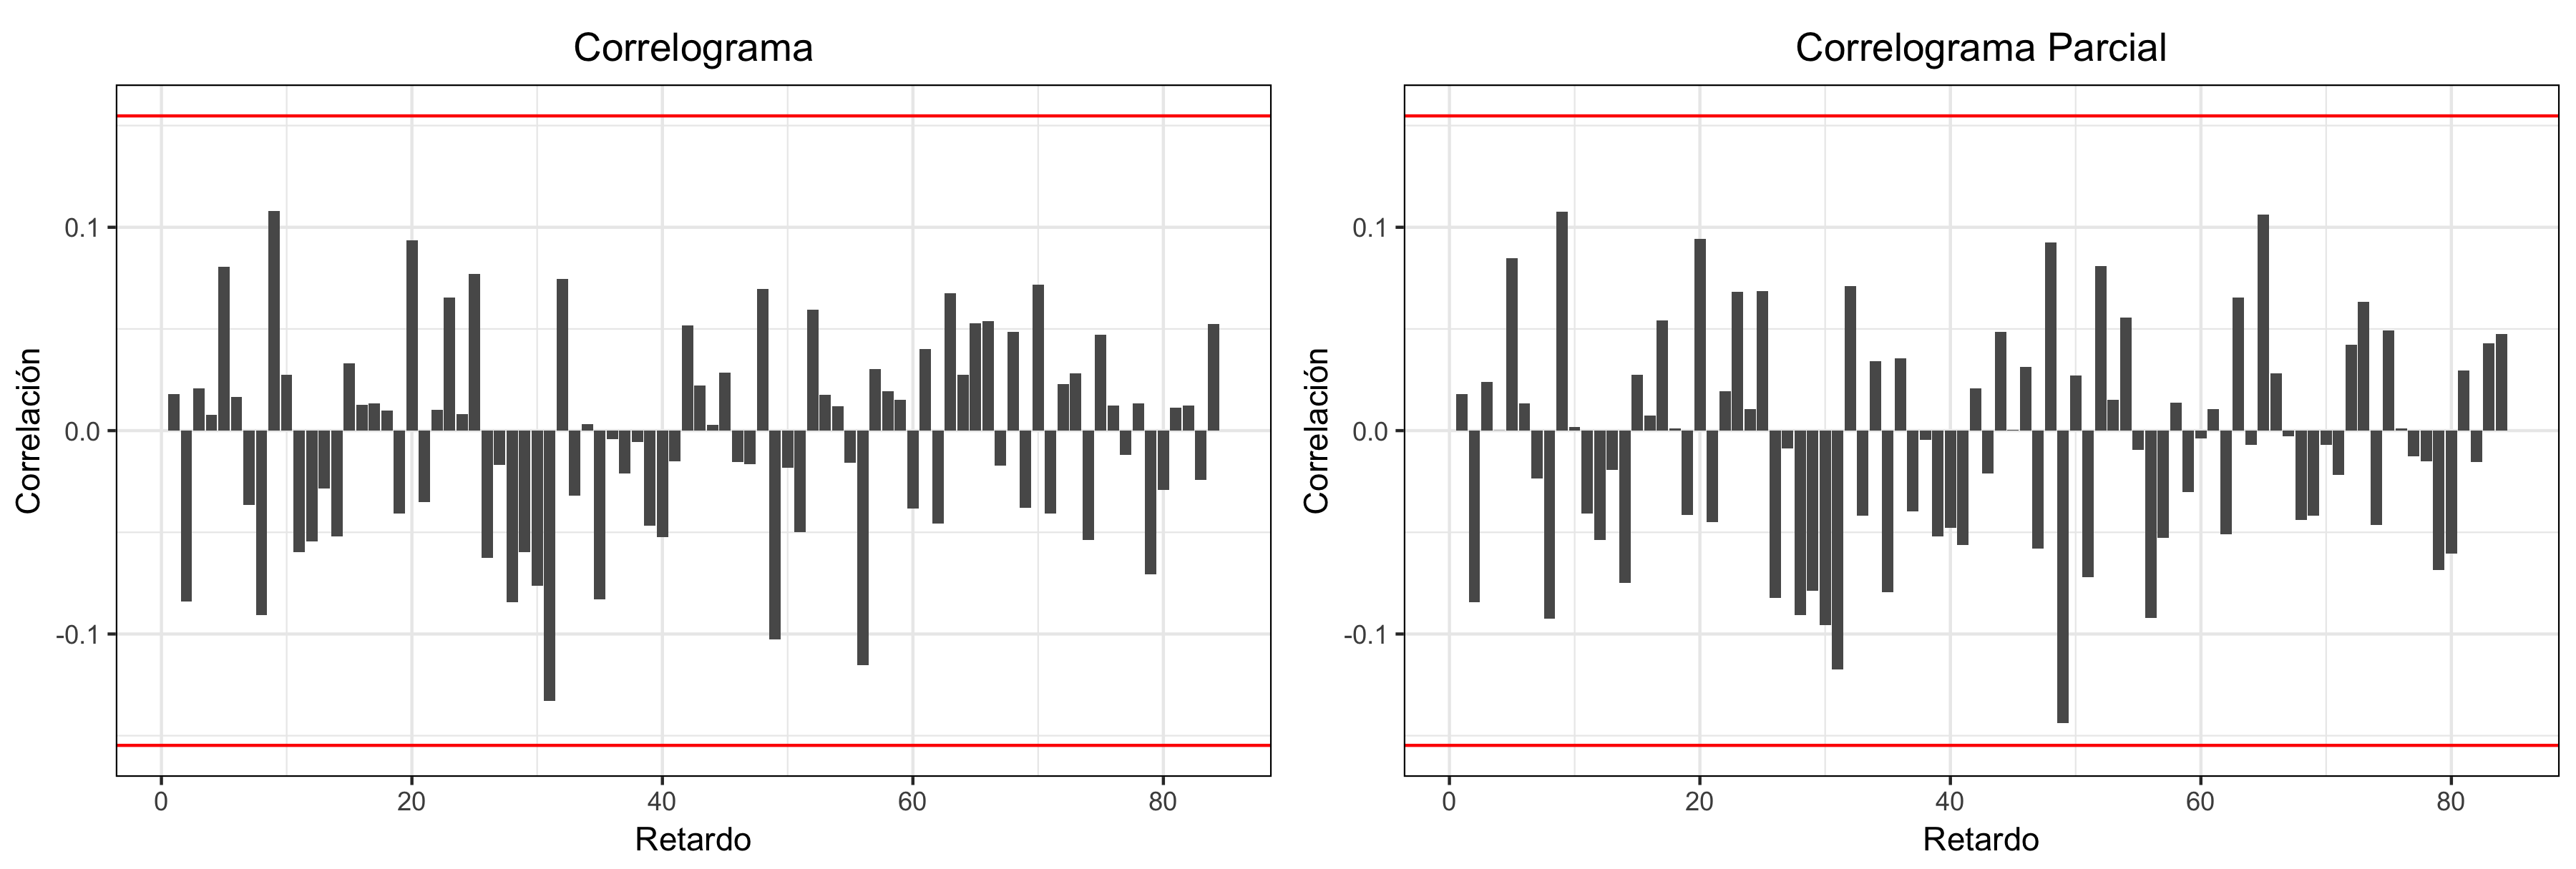
\includegraphics[width=\textwidth]{validation-2-acf-pacf}
    \end{figure}

    \item \textbf{Contrastes de Portmanteu}:
    \begin{table}[H]
      \begin{verbatim}
        Box-Ljung test
        X-squared = 0.055242, lag = 1, p-value = 0.8142

        Box-Ljung test
        X-squared = 7.6285, lag = 12, p-value = 0.8134
      \end{verbatim}
    \end{table}

  \end{itemize}
\end{document}